% This template has been downloaded from:
% http://www.latextemplates.com
%
% Original author:
% Ted Pavlic (http://www.tedpavlic.com)
%
% Modified by:
% Charles Newey (http://assemblyco.de)
%----------------------------------------

% Declare document
\documentclass{article}

% Packages
\usepackage{fancyhdr} % Required for custom headers
\usepackage{lastpage} % Required to determine the last page for the footer
\usepackage{extramarks} % Required for headers and footers
\usepackage{graphicx} % Images
\usepackage{tabularx} % Tables
\usepackage[table]{xcolor} % Table colours
\usepackage[colorlinks]{hyperref} % For URLs
\usepackage[T1]{fontenc} % Support symbols like < and >
\usepackage{lmodern} % Format symbols properly

% Colours
\definecolor{negligible}{rgb}{0.55, 0.71, 0.0}
\definecolor{acute}{rgb}{1.0, 0.75, 0.0}
\definecolor{severe}{rgb}{1.0, 0.49, 0.0}
\definecolor{critical}{rgb}{0.9, 0.17, 0.31}

% Margins
\topmargin=-0.45in
\evensidemargin=0in
\oddsidemargin=0in
\textwidth=6.5in
\textheight=9.0in
\headsep=0.25in
\linespread{1} % Line spacing

% Other setup
\pagestyle{fancy}
\renewcommand\headrulewidth{0.4pt} % Size of the header rule
\renewcommand\footrulewidth{0.4pt} % Size of the footer rule
\setlength\parindent{0pt} % Removes all indentation from paragraphs
\renewcommand{\refname}{} % Removes bibliography title

% Set up constants
\newcommand{\address}{
\small{
	\begin{tabular}{ l}
		Department of Computer Science, \\
		Llandinam Building, \\
		Aberystwyth University, \\
		Aberystwyth, \\
		Ceredigion, \\
		SY23 3DB \\
	\end{tabular}
	}
}

% Set up the header and footer
\lhead{\doctitle}										% Top left header
\chead{\version}											% Top center head
\rhead{\firstxmark \status}								% Top right header
\lfoot{\lastxmark \qanumber}								% Bottom left footer
\cfoot{Aberystwyth University/Computer Science}			% Bottom center footer
\rfoot{Page\ \thepage\ of\ \protect\pageref{LastPage}}	% Bottom right footer

% Set up title page
\title{
	\vspace{1.2in}
	\textmd{\textbf{\doctitle}} \\
	\vspace{0.1in}\large{\textit{\today}} \\
	\vspace{0.4in}
	{\bf{\qanumber}} \\ \vspace{0.4in} % QA document number
	\version \\
	\status \\
	\vspace{0.4in}
}

\author{\authors}
\date{}


%----------------------------- UPDATE THESE FOR EACH DOCUMENT ------------------------------
\newcommand{\version}{Version: 1.2}
\newcommand{\status}{Status: Release}
\newcommand{\qanumber}{SE.10.D1}
\newcommand{\doctitle}{Group 10 Project Plan}

\newcommand{\authors}{ % Include a table for authors
	\begin{tabular}{| l | l |}
		\hline
		\bf{Contributor Name} & \bf{Role} \\
		\hline
		Daniel Clark & Project Lead \\
		\hline
		Mark Lewis & QA Manager \\
		\hline
		Charles Newey & Deputy Project Lead \& Android Developer \\
		\hline
		Martin Ferris & Android Developer \\
		\hline
		Ashley Iles & Android Developer \\
		\hline
		Kenny Packer & Android Developer \\
		\hline
		Stephen McFarlane & Deputy QA \& Web Developer \\
		\hline
		Kieran Palmer & Web Developer \\
		\hline
	\end{tabular}
	% Don't edit this
	\\ \\ \\ \\ \\ \\
	\address \vline
	\hspace{0.15in} \copyright Copyright Group 10, 2013
	% Don't edit this
}

% Make title page, ToC and other introductory elements
\begin{document}
	\maketitle
	\newpage
	\tableofcontents
	\newpage

	% Begin the actual document
	%-------------------------------------- DOCUMENT STARTS HERE ------------------------------------
	\begin{section}{INTRODUCTION}
		\begin{subsection}{Purpose of This Document}
			The purpose of this document is to show that we have met the outlined objectives specified by the client. 

The main objective of the project is to create an application to compile and process data based on a walking tour. The data will be stored in a database which is sent data from a mobile application. The mobile application will guide people around the walk, showing them places of interest along the route. The application will be able to build a number of walks, showing the locaton and details of places of interest such as a short description, long description and photo about each point. All textual data will be stored in English.

The main objective quoted as follows: "Walking Tour Creator (WTC) is a computer-based system to compile data about a walking tour, and structure it in a database that can be used by a mobile application which guides people around the walk, showing them places of interest along the way. WTC will be able to build a number of related walks, showing the location and details of places of interest along with photos, audio, video, about each place. All textual data will be stored in English." \\
Reference: B. P. Tiddeman (2013), Software Engineering Group Projects – Project Plan Specification Standards 

This document will show we have managed to simplify these into a set of manageable goals. Gantt charts and GitHub's contribution analysis functionality will be used in conjunction to show and monitor the progress of the project's major tasks and other milestones. We are also implementing a risk analysis system that should alert us to the various problems that we may face whilst completing our objectives, and also allow us to mitigate the risks involved.
		\end{subsection}
	
		\begin{subsection}{Scope}
			This document should take into account the specifications of the project. This document includes an overview of our proposed systems - which will encompass our choice of platforms, some high-level architectures and a description of prospective users. The document also contains; a use case diagram giving an overview of how the app and the web systems will interact, mock-ups and descriptions of the UI design and how both applications will interact with the user, a Gantt chart which displays the start and end dates for the main milestones, and a risk analysis for the project.
		\end{subsection}
		
		\begin{subsection}{Objectives}
			These main objectives are to show our initial plans for the project. These goals include an overview of our proposed system, a set of use case diagrams, user interface designs, a Gantt chart, and a risk analysis.
			
			\begin{itemize}
				\item{Produce an overview of our proposed system, which matches our client's specifications.}
				\item{Produce a set of detailed use case diagrams to define the interactions with the system components and users and provide them with a concise explanation, along with example usage scenarios.}
				\item{Create a UI for the Android and web systems we will employ, with a succinct explanation for our chosen design.}
				\item{Employ the usage of a Gantt chart, to document our expected progress as a team.}
				\item{Highlight aspects of our project plan which may cause us difficulties in completing our assigned work in a timely manner.}
			\end{itemize}
		\end{subsection}
	\end{section}

	\newpage
	\begin{section}{SYSTEM OVERVIEW}
		\begin{subsection}{Introduction}
			Our proposed system is an application that will allow the user to create guided tour, with waypoints that include photographs and descriptions. We will implement the ability to record new routes via an Android interface and view previously recorded routes via a web interface.
		\end{subsection}
		
		
		\begin{subsection}{High Level Architecture Diagram}
			\begin{figure}[h!]
				\begin{center}
					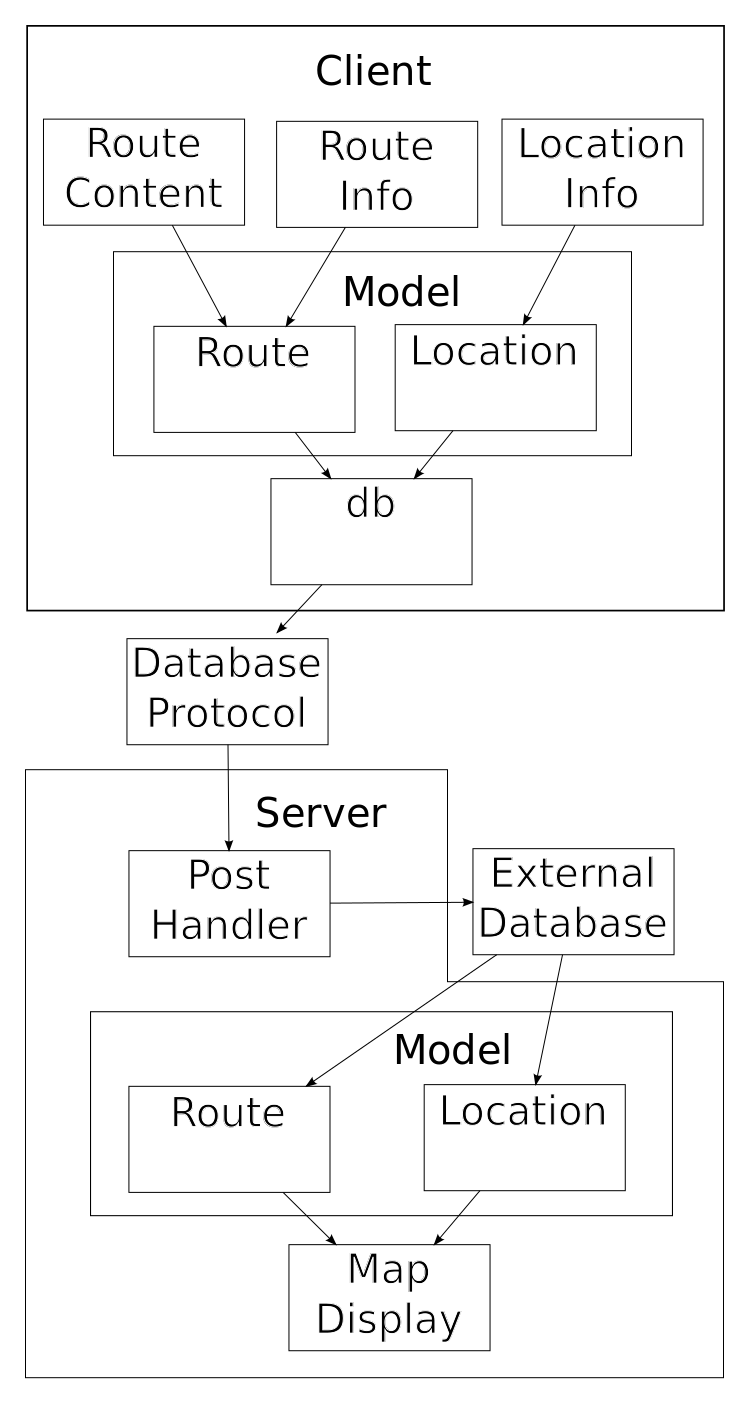
\includegraphics[height=\columnwidth]{./Diagrams/HighLevelArchitecture/HighLevelArchitecture.png}
				\end{center}
				\caption{A diagram showing the high-level architecture of the system.}
			\end{figure}
		\end{subsection}
				
		\clearpage
		\begin{subsection}{Client and Server Languages}
			The server will use a MySQL database as backend and a PHP, HTML, and JavaScript frontend. The Android application will use Java and the associated Google APIs as programming languages.
		\end{subsection}
	\end{section}
	
	\begin{section}{Platforms and High Level Architecture}
		\begin{subsection}{Mobile Architecture}
			\begin{subsubsection}{Operating System}
				It is stated in the specification set by the client that the system is to be designed for Android mobile phones.
			\end{subsubsection}
			
			\begin{subsubsection}{Location Derivation}
				The user's location will primarily be derived over GPS, but also may be derived from WiFi and Cell network, using Google's Location API, a functionality which is present within Android.
			\end{subsubsection}
			
			\begin{subsubsection}{Connectivity}
				The application will need to use several aspects of a mobile phone's connectivity - for a start, when the user is creating a walk, each waypoint will need to be marked with GPS coordinates. Then a further functional requirement specifies that the application must be able to upload each route in an HTTP POST to a remote server. This obviously requires the utilisation of internet connectivity - the application will support uploading over both WiFi (or 802.11 Wireless LAN) and over the mobile network. \\
				
				Being able to upload over WiFi and the mobile network introduces problems with the upload of the "route package" - uploading over the mobile network will take considerably longer than over WiFi, not to mention increasing the impact on the user's battery life. Because of this the system will be designed to alter the size and quality of each image within the route package, based on connection type. If the mobile network is being used (rather than WiFi), then the images will be "shrunk" in size and the JPEG compression will be slightly increased to compensate for the connection difference. \\
				
				The problem of connection instability must also be addressed. The application must be robust enough to reliably deliver a finished route over HTTP - a problem when using a mobile network or WiFi. The application will be able to handle connection outages and instability, and subsequently resume or retry transmission when a stable connection is restored.
			\end{subsubsection}
			
			\begin{subsubsection}{Usage of Other Hardware}
				The application must be able to attach photos for each waypoint along the route. These photos will be accessible either through the device's camera, or through the device's gallery. This means that some Android API calls must be used to be able to access the camera functionality and the device's file system.
			\end{subsubsection}
		\end{subsection}
		
		\clearpage
		\begin{subsection}{Web Architecture}
			\begin{subsubsection}{Server-Side Scripting}
				PHP is the chosen server-side scripting language. It is sufficiently fast and light enough to serve our needs, and has a reputation for stability. PHP is also excellent for HTML page generation, MySQL database integration, and page updating via asynchronous technologies like AJAX.
			\end{subsubsection}
			
			\begin{subsubsection}{Client-Side Scripting}
				For more dynamic areas of the web interface, and client-side access to some of the APIs provided by Google, we will be using Javascript. As part of the extended functionality there may also be AJAX implemented in the web interface, which will help the user retrieve walks from a search function.
			\end{subsubsection}
			
			\begin{subsubsection}{Database}
				MySQL is a popular and widely used database platform which will be used to store the data from each route. This will be used as a backend for both the Android application's upload function, and the web interface.
			\end{subsubsection}			
			
			\begin{subsubsection}{APIs}
				A large part of the web interface's codebase will revolve around generating a map with the Google Maps API. The API will allow us to dynamically generate a map containing the waypoints for each route.
			\end{subsubsection}

			\begin{subsubsection}{Android Version}
				The android SDK version we are using is 8. This will allow our application to run on any android devices running version 2.2 or higher.
		\end{subsection}
	\end{section}
	
	\newpage
	\begin{section}{GANTT CHART}
		\begin{center}
		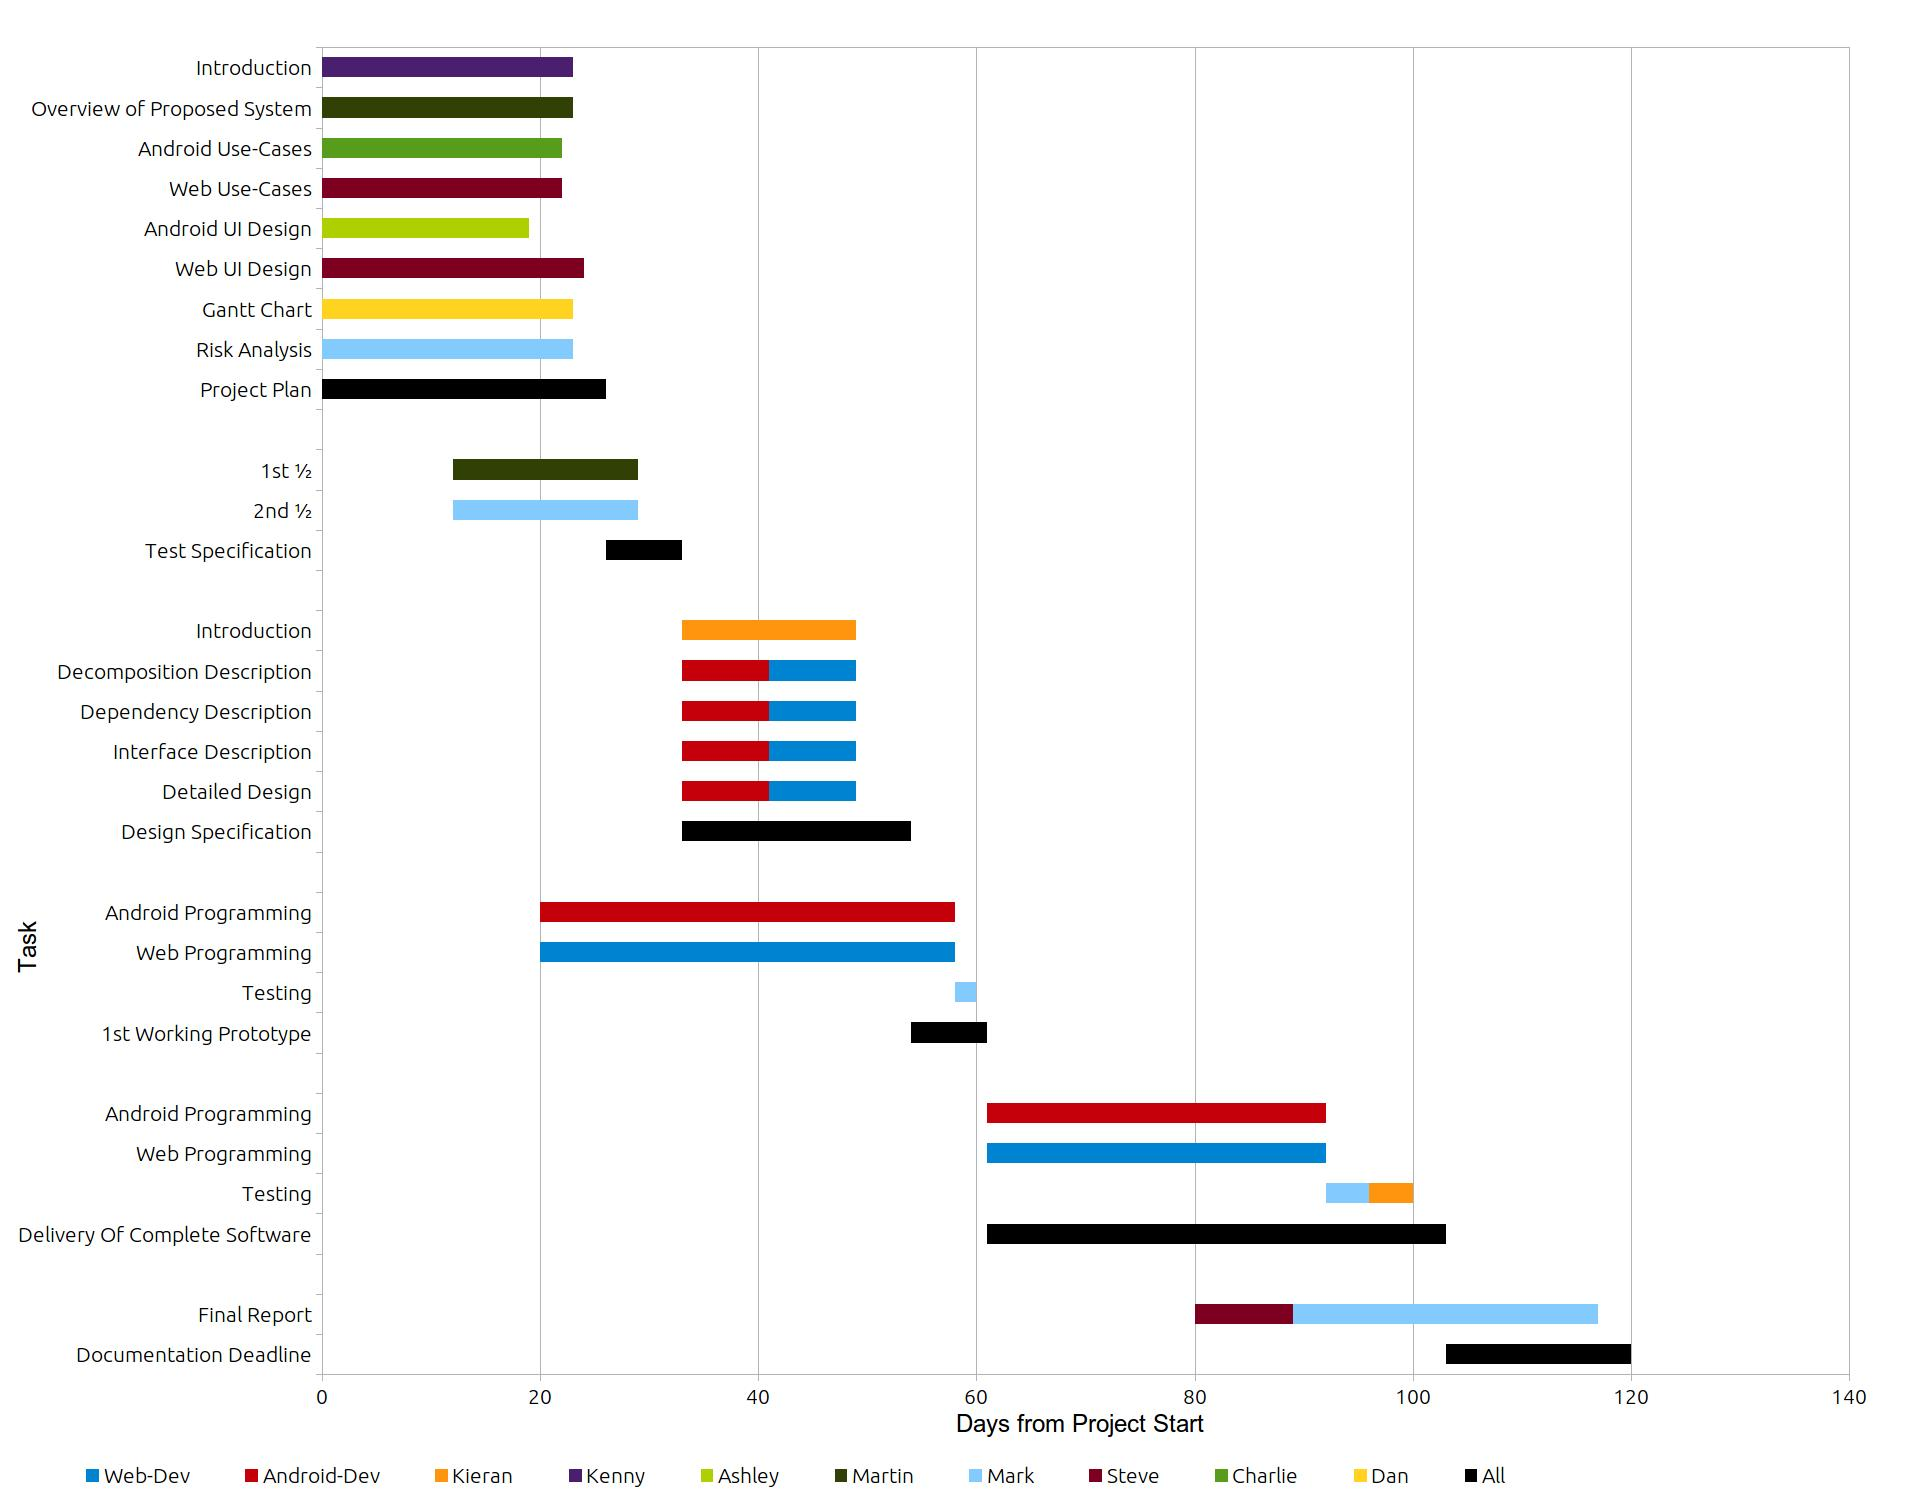
\includegraphics[height=1\columnwidth, angle=90]{./Diagrams/GanttChart/GanttChart.jpg}
		\end{center}
	\end{section}
	
	\newpage
	\begin{section}{RISK ANALYSIS}
		\begin{subsection}{Ongoing Tasks}
			\begin{tabularx}{\linewidth}{| p{3.5cm} | p{0.5cm} | p{0.5cm} | p{0.8cm} | X |}
				\hline
				\bf{Risk Event} & \bf{L} & \bf{M} & \bf{Risk} & \bf{Mitigation} \\
				\hline
				Team member absence & 0.6 & 0.3 & \cellcolor{green} 0.18 & All team members to regularly check emails and the agreed online resources for meeting times. Being unaware of meetings is not a valid excuse. If a team member is unable to attend a meeting, the project lead (Daniel) must be notified as soon as they know they can't attend. \\
				\hline
				Project Lead absence & 0.6 & 0.5 & \cellcolor{negligible} 0.30 & Meeting to go ahead as planned with Charlie (Deputy Project Lead) taking the meeting. \\
				\hline
				QA Manager absence & 0.6 & 0.3 & \cellcolor{green} 0.18 & Meeting to go ahead as planned with Steve (Deputy QA Manager). \\
				\hline
				Unable to contact team member & 0.3 & 0.8 & \cellcolor{negligible} 0.24 & Ensure that all team members regularly check emails and other agreed online resources, as well as checking meeting minutes so they are aware of any outstanding tasks/actions. Persistently being unreliable with result in a warning, and further action if necessary; e.g. carding or role reallocation. \\
				\hline
				Git failure & 0.3 & 1.0 & \cellcolor{negligible} 0.3 & All work to be backed up regularly in several places in case of human error or Git failure. \\
				\hline
				Major illness or unexpected circumstances & 0.5 & 0.9 & \cellcolor{acute} 0.45 & Team members to be notified as soon as possible, in case any urgent tasks need to be re-assigned or completed by another team member. \\
				\hline
				Git conflict & 0.3 & 0.9 & \cellcolor{negligible} 0.27 & All team members are to have read the information on the project wiki on Git conflicts. If a conflict is encountered, then it must be resolved immediately. If a conflict cannot be resolved easily, then an appropriate team member (Git expert/project lead) must be notified and the conflict must be resolved. Try to ensure an even task allocation, to avoid multiple team members working on the same code simultaneously. \\
				\hline
			\end{tabularx}
		\end{subsection}
		\definecolor{applegreen}{rgb}{0.55, 0.71, 0.0}
		\begin{subsection}{Documentation}
			\begin{tabularx}{\linewidth}{| p{3.5cm} | p{0.5cm} | p{0.5cm} | p{0.8cm} | X |}
				\hline
				\bf{Risk Event} & \bf{L} & \bf{M} & \bf{Risk} & \bf{Mitigation} \\
				\hline
				Late submission & 0.4 & 0.8 & \cellcolor{negligible} 0.32 & Deadlines for documentation to be brought forward to ensure that any future problems encountered will come to light within a reasonable time frame. If team members run into any problems, they are to alert the group so that a solution can be issued. \\
				\hline
				Inadequate quality submission & 0.4 & 1.0 & \cellcolor{acute} 0.4 & Documents to be checked by either of the QA managers or project leaders before submitting. If team members need help then they should ask the rest of the team for help. \\
				\hline
				Human error & 0.5 & 0.2 & \cellcolor{green} 0.1 & All documents to be checked for spelling, grammar, logic, and clerical errors by the creator of each document and at least one other team member. \\
				\hline
				Loss of documentation & 0.4 & 1.0 & \cellcolor{acute} 0.4 & Documentation to be stored and versioned on Git and backed up individually by the document's creator. Each individual is responsible for their own documentation. \\
				\hline
			\end{tabularx}
		\end{subsection}
		
		\newpage
		\begin{subsection}{Software Development}
			\begin{tabularx}{\linewidth}{| p{3.5cm} | p{0.5cm} | p{0.5cm} | p{0.8cm} | X |}
				\hline
				\bf{Risk Event} & \bf{L} & \bf{M} & \bf{Risk} & \bf{Mitigation} \\
				\hline
				Project behind schedule & 0.5 & 1.0 & \cellcolor{acute} 0.5 & Development to begin as soon as possible. Charlie (lead developer) to delegate any appropriate outstanding tasks. Regular feedback to be given by Daniel (project lead) to ensure schedule is adhered to. \\
				\hline
				Parts of the project missing/incomplete & 0.4 & 1.0 & \cellcolor{acute} 0.4 & Daniel (project lead) and Charlie (lead developer) to delegate programming tasks appropriately. Constant testing by QA managers and project leaders to check if code is of a sufficient quality. \\
				\hline
			\end{tabularx}
		\end{subsection}
		
		\begin{subsection}{Risk Grade and Recommended Action Key}
			\begin{tabularx}{\linewidth}{| X | X | X | X | X | X | X | X |}
				\hline
				\bf{Risk Grade} & Less than negligible & Negligible & Acute & Severe & Critical & Catastrophic \\
				\hline
				\bf{Risk score} & \cellcolor{green} < 0.2 & \cellcolor{negligible} 0.2 - 0.39 & \cellcolor{acute} 0.4 - 0.59 & \cellcolor{severe} 0.6 - 0.79 & \cellcolor{critical} 0.8 - 0.99 & \cellcolor{red} 1.0 \\
				\hline
				\bf{Action} & Tolerate & Tolerate & Tolerate or treat & Treat & Transfer & Terminate \\
				\hline
			\end{tabularx}
		\end{subsection}
	\end{section}
	
	\begin{section}{USE CASES AND SCENARIOS}
		\begin{subsection}{Overview of Use Cases}
			\begin{subsubsection}{Core Functionality}
				The "core functionality" sections represent the highest priority features for the project, and will be the bare minimum functionality that the project will contain.
			\end{subsubsection}
			
			\begin{subsubsection}{Extended Functionality}
				The "extended functionality" sections represent the lower priority features, that will be implemented within the project if time permits.			
			\end{subsubsection}
		\end{subsection}
		
		\clearpage
		\begin{subsection}{Android - Core Functionality}
			\begin{subsubsection}{Create Route}
				\begin{figure}[h!]
					\begin{center}
						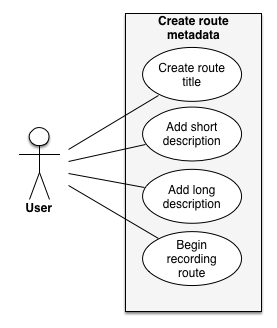
\includegraphics[height=0.55\columnwidth]{./Diagrams/UseCase/Android/Core/CreateRoute.png}
					\end{center}
					\caption{A user wants to create a new walk. The user will progress from the main screen to the "create route" screen, and fill in the route title, a short description (a tagline), and a long description. From there, the user can progress to recording the route.}
				\end{figure}
			\end{subsubsection}
			
			\clearpage
			\begin{subsubsection}{Record Route}
				\begin{figure}[h!]
					\begin{center}
						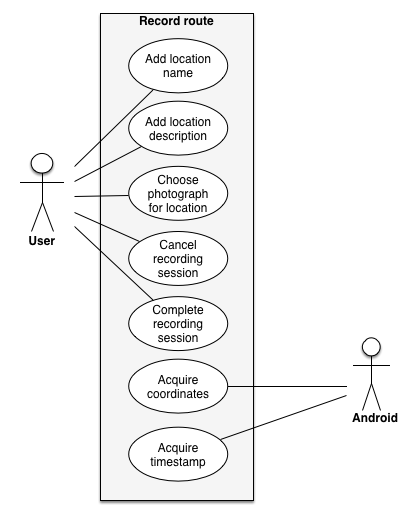
\includegraphics[height=0.75\columnwidth]{./Diagrams/UseCase/Android/Core/RecordRoute.png}
					\end{center}
					\caption{At each location (or waypoint) that the user chooses, they will retrieve their phone and enter the name and a description for the location. A photo can also be chosen from the gallery or taken using the camera - and then added to the waypoint. From this screen, the user can choose to complete the recording session, or cancel it entirely. The Android device will automate the task of fetching GPS coordinates and attaching a timestamp to each entry.}
				\end{figure}
			\end{subsubsection}
			
			\clearpage
			\begin{subsubsection}{Complete Route}
				\begin{figure}[h!]
					\begin{center}
						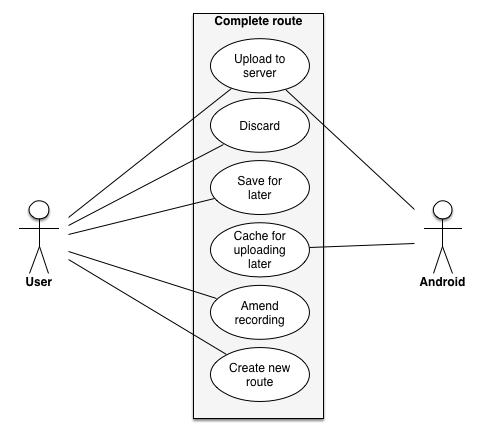
\includegraphics[height=0.7\columnwidth]{./Diagrams/UseCase/Android/Core/CompleteRoute.png}
					\end{center}
					\caption{After the user has entered all of the locations that they wish to add and elected to complete the recording, they will be presented with several choices. They can upload the changes to the server (this will be handled by the Android system), saving the walk for later, discarding the walk entirely, or amending the recording - in case a mistake was made. The Android system will also be able to cache the recording for later upload (in the case of no signal, or other upload errors). The user will also be able to create a new route from this screen.}
				\end{figure}
			\end{subsubsection}
			
			\clearpage
			\begin{subsubsection}{System}
				\begin{figure}[h!]
					\begin{center}
						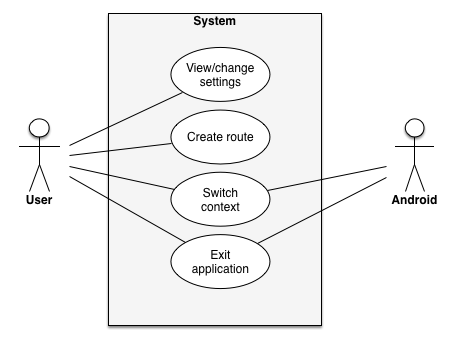
\includegraphics[height=0.55\columnwidth]{./Diagrams/UseCase/Android/Core/System.png}
					\end{center}
					\caption{The user will be able to view or change their default settings and create a route from this screen. The application will also be able to handle context switching (i.e. switching to another app) and the application will be able to handle exits safely.}
				\end{figure}
			\end{subsubsection}
		\end{subsection}
		
		\clearpage
		\begin{subsection}{Android - Extended Functionality}
			\begin{subsubsection}{Create Route}
				\begin{figure}[h!]
					\begin{center}
						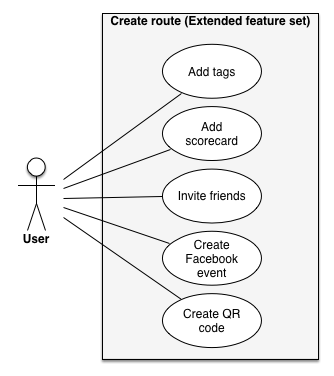
\includegraphics[height=0.55\columnwidth]{./Diagrams/UseCase/Android/Extended/CreateRoute_Extended.png}
					\end{center}
					\caption{The user will be able to 'tag' their walk(s) with keywords to aid searching on the website. The user will be able to create a Facebook event (through a Facebook app), and invite friends to such an event. Another function available would be to generate a QR code to the Facebook event URL, to help the user share the event effectively.}
				\end{figure}
			\end{subsubsection}
			
			\begin{subsubsection}{Record Route}
				\begin{figure}[h!]
					\begin{center}
						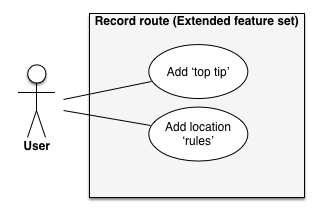
\includegraphics[height=0.3\columnwidth]{./Diagrams/UseCase/Android/Extended/RecordRoute_Extended.png}
					\end{center}
					\caption{The user will be able to add a 'top tip' for every location; for example, a favourite drink or best place to sit. The user will also be able to choose 'rules' for each location for the followers of the walk - so as to allow the participants of the walk to play a game, or complete a challenge.}
				\end{figure}
			\end{subsubsection}
			
			\clearpage
			\begin{subsubsection}{Complete Route}
				\begin{figure}[h!]
					\begin{center}
						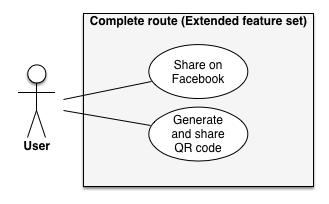
\includegraphics[height=0.3\columnwidth]{./Diagrams/UseCase/Android/Extended/CompleteRoute_Extended.png}
					\end{center}
					\caption{The user will be able to choose to share the create event on Facebook using a Facebook app, as well as sharing the QR code generated earlier.}
				\end{figure}
			\end{subsubsection}
			
			\begin{subsubsection}{System}
				\begin{figure}[h!]
					\begin{center}
						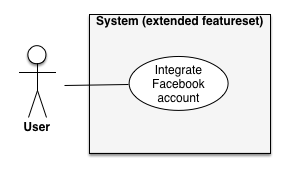
\includegraphics[height=0.3\columnwidth]{./Diagrams/UseCase/Android/Extended/System_Extended.png}
					\end{center}
					\caption{The user will be able to integrate the application with their Facebook account (using a Facebook app and OAuth authentication).}
				\end{figure}
			\end{subsubsection}
		\end{subsection}
		
		\clearpage
		\begin{subsection}{Website - Core Functionality}
			\begin{subsubsection}{System}
				\begin{figure}[h!]
					\begin{center}
						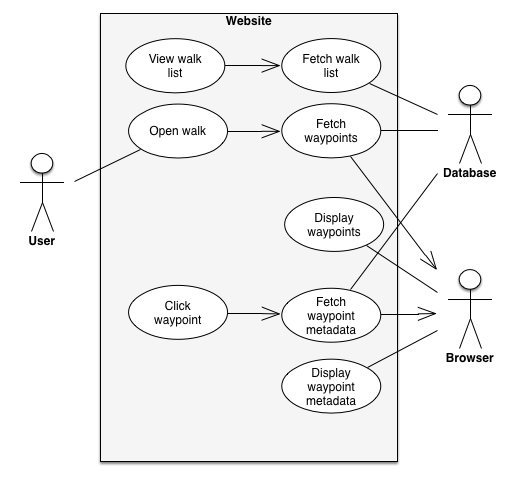
\includegraphics[height=0.75\columnwidth]{./Diagrams/UseCase/Website/Core/Website.png}
					\end{center}
					\caption{When the page loads, the user will be prompted with a list of walks to load. This will be achieved by the webpage querying the database - the database will provide the information and display it to the user in the browser. The user will be able to open a walk using the web interface, and this will request the walk's information from the database and cause the browser to display the information for each walk on a map. Upon the user clicking a waypoint on the map, the information for each waypoint will be fetched from the database and displayed on-screen.}
				\end{figure}
			\end{subsubsection}
		\end{subsection}
		
		\clearpage
		\begin{subsection}{Website - Extended Functionality}
			\begin{subsubsection}{System}
				\begin{figure}[h!]
					\begin{center}
						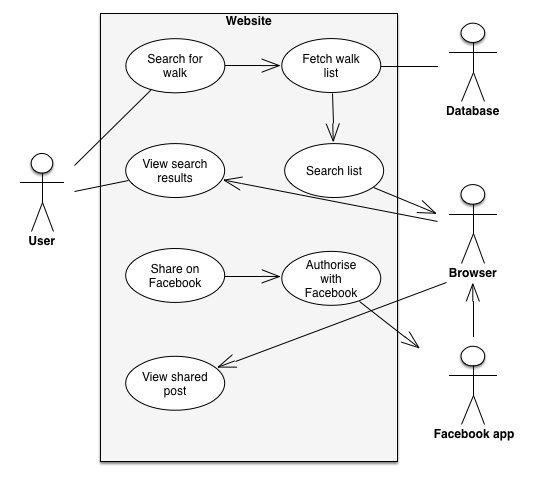
\includegraphics[height=0.75\columnwidth]{./Diagrams/UseCase/Website/Extended/Website.png}
					\end{center}
					\caption{The user will be able to search for walks within the browser, which will search through the database and display the matching walks. The user will also be able to share walks on Facebook using a Facebook app.}
				\end{figure}
			\end{subsubsection}
		\end{subsection}
	\end{section}
	
	\clearpage
	\begin{section}{USER INTERFACE DESIGNS}
		\begin{subsection}{Android Interface Designs}
			\begin{subsubsection}{Home}
				\begin{figure}[h!]
					\begin{center}
						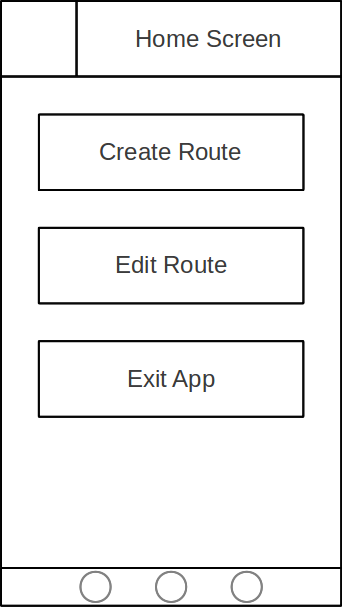
\includegraphics[height=0.45\columnwidth]{./Diagrams/AndroidUserInterface/source/homeScreen.png}
					\end{center}
					\caption{The home screen is the first screen that the user will be able to see when the app is loaded. There are three buttons on this page the first two will, when clicked, take the user to the Route Info or Unfinished Route screen. The last button on this screen will close the application.}
				\end{figure}
			\end{subsubsection}
			
			\clearpage
			\begin{subsubsection}{Create Route}
				\begin{figure}[h!]
					\begin{center}
						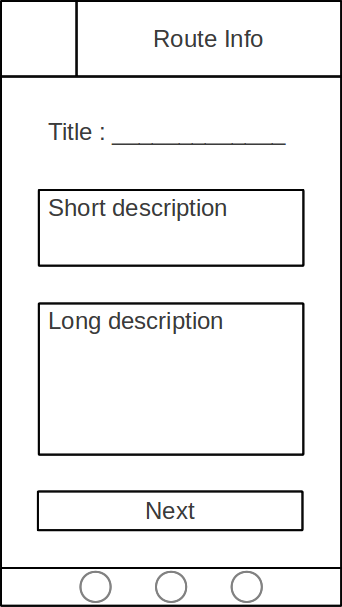
\includegraphics[height=0.45\columnwidth]{./Diagrams/AndroidUserInterface/source/routeInfo.png}
					\end{center}
					\caption{When the user wants to create a new route this is the next screen that they will encounter. The three text boxes will allow the user to enter the route's identifier (title) as well as descriptive information about the route. At the bottom of the screen is the next button that will allow the user to progress the the Route Content screen.}
				\end{figure}
			\end{subsubsection}
			
			\clearpage
			\begin{subsubsection}{Add Waypoint}
				\begin{figure}[h!]
					\begin{center}
						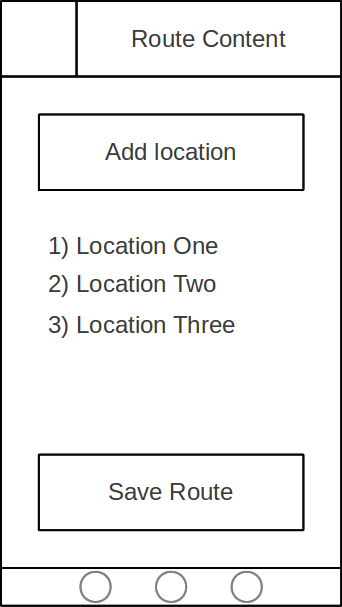
\includegraphics[height=0.45\columnwidth]{./Diagrams/AndroidUserInterface/source/routeContent.png}
					\end{center}
					\caption{On this screen the user can add locations of interest to the route by clicking on the Add Location button, this action will also take the user to the Location Info screen. After a location has been added it will appear in the list of locations underneath the Add Location button. When the user is finished adding locations to the route they can click on the Save Route button, at this point they will be prompted as to weather they wish to upload to the server or save the route locally for editing later.}
				\end{figure}
			\end{subsubsection}
			
			\clearpage
			\begin{subsubsection}{Location Information}
				\begin{figure}[h!]
					\begin{center}
						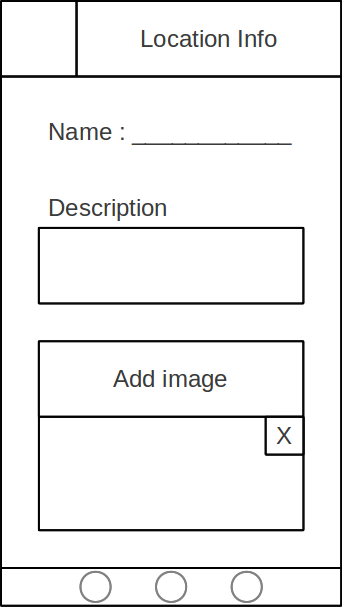
\includegraphics[height=0.45\columnwidth]{./Diagrams/AndroidUserInterface/source/locationInfo.png}
					\end{center}
					\caption{The name and description can be entered into text boxes on this screen. Also images of the location can be added using the Add Image button. Images that have been added will be displayed below the Add Image button, and below the image place holder is the Save button that will return the user to the Route Content screen.}
				\end{figure}
			\end{subsubsection}
			
			\begin{subsubsection}{Unfinished Routes}
				\begin{figure}[h!]
					\begin{center}
						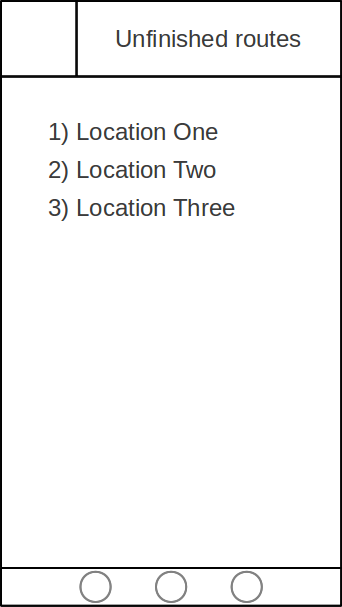
\includegraphics[height=0.45\columnwidth]{./Diagrams/AndroidUserInterface/source/unfinishedRoutes.png}
					\end{center}
					\caption{This screen will list the routes that have been saved locally but not uploaded to the sever. When an item in the list is clicked on the user will be taken to the Route Info page for that item so that they can edit it's content.}
				\end{figure}
			\end{subsubsection}
		\end{subsection}
		
		\clearpage
		\begin{subsection}{Web Interface Designs}
			\begin{subsubsection}{Main Web Interface}
				\begin{figure}[h!]
					\begin{center}
						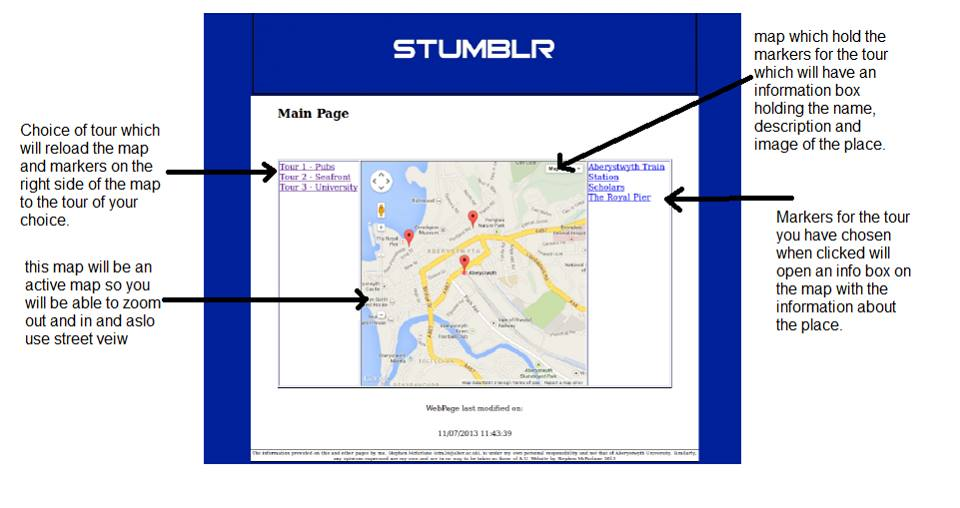
\includegraphics[height=0.55\columnwidth]{./Diagrams/WebUserInterface/AnnotatedUI.jpg}
					\end{center}
					\caption{This is a sample UI for the tour viewer;  The design of the final page might be different.}
				\end{figure}
			\end{subsubsection}
		\end{subsection}
	\end{section}

	% Include references here (edit the References.bib file)
	\nocite{LaTeXTemplate}

	% Format bibliography/refs
	\newpage
	\begin{section}{REFERENCES}
		\bibliographystyle{acm}
		\bibliography{References}
	\end{section}
	
	\vspace{1cm}
	\begin{section}{VERSION HISTORY}
		\begin{tabularx}{\linewidth}{| p{2cm} | p{2cm} | p{2cm} | X | }
			\hline
			\bf{Author} & \bf{Date} & \bf{Version} & \bf{Change made} \\
			\hline
			CCN & 07/11/2013 & 1.1 & Updated order of authors on cover \\
			\hline
			DEC & 07/11/2013 & 1.2 & Added High Level Architecture diagram \\
			\hline
		\end{tabularx}
	\end{section}
\end{document}

%									Useful bits and pieces
%\begin{section}{section_name}								% Start section
%\end{section}												% End section
%\begin{center} \end{center}								% Center stuff
%\includegraphics[width=0.75\columnwidth]{example_figure}	% Insert image
%\pseudocode{filename}{caption}								% Insert highlighted code snippet
%\clearpage													% Clear page after section
%\url{http://www.google.com/} 								% Include URL
%\nocite{citationName}										% Cite to bibliography (but not to text)
%\cite{citationName}										% Include reference